%%
% La siguiente plantilla esta basada en el siguiente enlace:
% http://academic.reed.edu/physics/courses/Physics332.s08/reports.html
% La plantilla original puede descargarse de ese sitio
% Se dejo parte del texto original en inglés para ilustar el uso de la plantilla
% Se hicieron algunas modificaciones para ajustar el idioma y otros detalles para 
% completar un reporte técnico breve pero muy puntual
% Modificación Inicial: Marco Aurelio Nuno Maganda - 11/SEP/2014
% 
% Enlace a la documentación del tipo de documento base (revtex4)
% http://mirror.hmc.edu/ctan/macros/latex/contrib/revtex/doc/latex/revtex/source/revtex4-1.pdf
%
% En algunas distribuciones es necesario instalar el paquete texlive-publishers
%
%\documentclass[letterpaper,aps,twocolumn,pre,nofootinbib]{revtex4}
%\documentclass[twocolumn]{article}
\documentclass[conference]{IEEEtran}

\usepackage[spanish]{babel}
\usepackage{amsmath,amssymb,amsfonts,amsthm}
\usepackage{graphicx}
%\usepackage{bbm}
\usepackage[utf8]{inputenc} % Caracteres en Español (Acentos, ñs)
\usepackage{url} % ACENTOS
\usepackage{hyperref} % Referencias
\usepackage{subfig}
\usepackage{lipsum}
\usepackage{balance}


\usepackage{graphicx} % Required for including images
\usepackage[font=small,labelfont=bf]{caption} % Required for specifying captions to tables and figures


\usepackage{tikz}
\usetikzlibrary{automata, positioning, arrows}

%%%%%%%%%%%%%%%%%%%%%%%%%%%%%%%%%%%%%%%%%%%%%
% PARCHE PARA ELIMINAR LA FECHA DEL DOCUMENTO
% 
\usepackage{etoolbox}
\makeatletter
% \frontmatter@RRAP@format is responsible for the parentheses
\patchcmd{\frontmatter@RRAP@format}{(}{}{}{}
\patchcmd{\frontmatter@RRAP@format}{)}{}{}{}
%\renewcommand\Dated@name{}
\makeatother	
% FIN DEL PARCHE
% 
%%%%%%%%%%%%%%%%%%%%%%%%%%%%%%%%%%%%%%%%%%%%%

%%%%%%%%%%%%%%%%%%%%%%%%%%%%%%%%%%%%%%%%%%%%%
% PARCHE PARA PERMIRIR UTILIZAR BIBLATEX EN ESTA PANTLLA
%\PassOptionsToPackage{square,numbers}{natbib}
%\RequirePackage{natbib}  
%%%%%%%%%%%%%%%%%%%%%%%%%%%%%%%%%%%%%%%%%%%%%

\usepackage[backend=bibtex,sorting=none]{biblatex}
% Estas lineas permiten romper los hipervinculos muy largos !!!!
\setcounter{biburllcpenalty}{7000}
\setcounter{biburlucpenalty}{8000}
\addbibresource{references.bib}

% Actualiza en automático la fecha de las citas de internet a la fecha de la compilación del documento
\usepackage{datetime}
\newdateformat{specialdate}{\twodigit{\THEDAY}-\twodigit{\THEMONTH}-\THEYEAR}
\date{\specialdate\today}

% la sentencia \burl en las citas... 
\usepackage[hyphenbreaks]{breakurl}

\renewcommand\spanishtablename{Tabla}
\renewcommand\spanishfigurename{Figura}



\begin{document}

\newcommand{\breite}{0.9} %  for twocolumn
\newcommand{\RelacionFiguradoscolumnas}{0.9}
\newcommand{\RelacionFiguradoscolumnasPuntoCinco}{0.45}



\title{Reporte de Proyecto Grupal 3 \\Aplicación de Seguimiento Facial de Realidad Aumentada}

\author{\IEEEauthorblockN{González Reyes Carmen Rubí\IEEEauthorrefmark{1},
Guerrero Salazar Julissa Vianney\IEEEauthorrefmark{1},\\
Hernández Rodríguez Elías\IEEEauthorrefmark{1},
Martínez Ibarra César Eduardo\IEEEauthorrefmark{1} y 
Resendiz García Alex Emil\IEEEauthorrefmark{1}}
\IEEEauthorblockA{Ingeniería en Tecnologías de la Información\\
Universidad Politécnica de Victoria}
}
\maketitle



\begin{abstract} 

    Este proyecto de Realidad Aumentada para Android se desarrolló integrando ARCore y Sceneform para permitir la superposición de modelos 3D en rostros detectados. El proceso de desarrollo abarcó desde la configuración del entorno y la implementación técnica del seguimiento de rostros en tiempo real y la carga asíncrona de modelos en MainActivity.java, hasta la creación de una interfaz de usuario intuitiva para la selección de modelos en ModelSeleccionMenu.java y ModelMapAdapter.java. Como parte del ciclo de desarrollo de la aplicación de Realidad Aumentada que interactúa con hardware y software complejos, se realizaron pruebas exhaustivas en dispositivos móviles para verificar la correcta detección y seguimiento de rostros, la superposición precisa de modelos 3D y la funcionalidad del menú de selección.

\end{abstract}

\section{Introducción}
    En un mundo digital en constante evolución, la Realidad Aumentada (RA) se ha establecido como una herramienta versátil \cite{cadavieco2012realidad}. Sin embargo, su integración en dispositivos móviles a menudo presenta desafíos, desde la complejidad de la configuración técnica hasta la implementación de un seguimiento facial preciso \cite{bernal2018analisis}.

    La aplicación de la RA y el seguimiento facial es un campo de estudio activo, con diversos trabajos que exploran su potencial en distintos sectores. En el ámbito del transporte, se han desarrollado sistemas que utilizan la RA para superponer datos e indicadores directamente en el entorno\cite{moctezumaimplementacion}. De manera similar, en el sector educativo, se han implementado plataformas que emplean el reconocimiento facial para la gestión y el seguimiento de estudiantes, mejorando la seguridad y el control de asistencia\cite{castro2022sistema}.

    Este proyecto presenta una aplicación de RA para móviles, desarrollada en el entorno de Android Studio\cite{android_blog,big_nerd_ranch}, utilizando Java. La aplicación se basa en la integración de las bibliotecas ARCore\cite{ar_core} y Sceneform\cite{sceneform}, permitiendo la superposición de modelos 3D sobre rostros detectados en tiempo real a través de la cámara frontal del dispositivo\cite{android_studio,base_proyecto}.
    
\section{Desarrollo Experimental} 

    \subsection{Fase 1: Configuración de la Arquitectura y Entorno}

        El viaje de desarrollo de esta aplicación de Realidad Aumentada (RA) para Android comenzó con la configuración fundamental del proyecto. En el entorno de desarrollo Android Studio (AS), se sentaron las bases integrando las dependencias esenciales de ARCore y Sceneform en el archivo \textbf{build.gradle}. Esto fue crucial, ya que estas bibliotecas otorgan acceso a las interfaces de programación de aplicaciones necesarias para habilitar tanto la RA como la capacidad de renderizar modelos 3D. Paralelamente, se ajustó el \textbf{AndroidManifest.xml} para solicitar los permisos de cámara indispensables y declarar la compatibilidad con las características de ARCore, asegurando así que la aplicación pudiera interactuar correctamente con el hardware del dispositivo y la plataforma de RA. La organización de los recursos también fue un paso temprano y vital; se crearon las estructuras de caretas \textbf{assets/models} y \textbf{assets/texturas} para almacenar los archivos de modelos 3D en formato \textbf{.gib} y sus texturas asociadas, preparando el escenario para la carga de activos visuales.

    \subsection{Fase 2: Implementación del Core de RA (MainActivity.java)}

        Con la arquitectura establecida, el foco se trasladó a la implementación del núcleo de la experiencia de RA, principalmente dentro de \textbf{MainActivity.java}. Aquí, se inicializó la vista de RA obteniendo o añadiendo dinámicamente un \textbf{ArFrontFacingFragment} al diseño de la actividad. Este fragmento, un componente clave de Sceneform UX, asume la responsabilidad de gestionar la cámara frontal y orquestar la sesión de ArCore específicamente para el seguimiento de rostros. Una vez que el fragmento estuvo operativo, su método \textbf{onViewCreated} proporcionó acceso a la \textbf{ArSceneView}. En este punto, se ajustó la prioridad del renderizado de la transmisión de la cámara y, de manera fundamental, se registró un \textbf{setOnArgumentedFcaceUpdateListener}. Este oyente actúa como el conducto a través del cual ARCore comunica los eventos de detección de rostros o cambios en su estado de seguimiento, activando respuestas dentro de la aplicación. La carga de los modelos 3D se manejó de forma asíncrona utilizando \textbf{ModelRenderable.builder}, lo que permitió que la aplicación continuara respondiendo mientras los activos se cargaban en segundo plano. El uso de \textbf{CompletableFuture} facilitó la gestión de estas operaciones, asegurando que el modelo renderizado (faceModel) estuviera disponible para su uso una vez completada la carga y proporcionando un mecanismo para manejar posibles errores durante el proceso.\\

        La gestión del seguimiento de rostros orquestada por el método \textbf{onArgimentedFaceTrackingUpdate}, es donde la RA cobra vida. Cuando ARCore detecta un \textbf{AugmentedFace} con un estado \textbf{TRACKING}, la aplicación responde creando una instancia de \textbf{AugmentedFaceNode},  un nodo de Sceneform especializado diseñado para integrarse con datos de rostros aumentados. A este nodo se le asigna el \textbf{faceModel} cargado previamente utilizando \textbf{setFaceRegionRenderable}, preparando el modelo 3D para ser superpuesto en el rostro detectado. Se configuraron propiedades como \textbf{setShadorCaster} y \textbf{setShadowReceiver} para refinar el comportamiento de las sombras del modelo en la escena. Posteriormente, el \textbf{AugmentedFaceNode} se añade a la escena de la \textbf{ArSceneView}, integrando visualmente el modelo 3D con la transmisión de la cámara frontal. Para mantener un registro de los rostros rastreados y sus nodos correspondientes. Para mantener un registro de los rostros rastreados y sus nodos correspondientes, se utilizó un \textbf{HashMap}, mapeando cada \textbf{AugmentedFace} a su \textbf{AugmentedFaceNode} asociado para una fácil referencia y manipulación. Si el estado de seguimiento de un rostro cambia a \textbf{STOPPED}, el \textbf{AugmentedFaceNode} correspondiente se elimina cuidadosamente de la escena y del \textbf{HasMap}, liberando recursos y manteniendo la escena limpia. Adicionalmente, se incorporó la reproducción de audio mediante un \textbf{MediaPlayer}, permitiendo que un archivo de sonido específico se reprodujera condicionalmente cuando se seleccionara un modelo particular, añadiendo una capa extra de interactividad a la experiencia de RA.

    \subsection{Fase 3: Desarrollo del Menú de Selección de Modelos (ModelSeleccionMenu.java y ModelMapAdapter.java)}

        Paralelamente a la implementación del núcleo de RA, se desarrolló la funcionalidad del menú de selección de modelos, que abarca \textbf{ModelSelecionMenu.java} y \textbf{ModelMapAdapter.java}. La actividad \textbf{ModelSelectionMenu.java} fue diseñada para presentar a los usuarios las opciones de modelos 3D disponibles a través de un \textbf{GridView}. Se definió un \textbf{LinkedHashMap} (modelList) para almacenar la asociación entre los nombres de visualización de los modelos y los nombres de archivo \textbf{.glb} correspondientes, manteniendo el orden de las opciones. Se adjuntó un \textbf{OnItemClickListener} al \textbf{GridView}, permitiendo que la aplicación respondiera cuando un usuario seleccionara un modelo. Tras la selección, se obtuvo el nombre del archivo del modelo elegido y se comunicó de vuelta al \textbf{MainActivity} utilizando un \textbf{Intent}, señalando el resultado de la selección y finalizando la actividad del menú. Para gestionar la visualización de los modelos en el \textbf{GridView}, se creó un adaptador personalizado, \textbf{ModelMapAdapter.java}, que extiende \textbf{BaseAdapter}. En su método \textbf{getView()}, este adaptador se encarga de inflar un diseño (\textbf{model\_item.xml}) para cada elemento del \textbf{GridView} asignando el nombre del modelo a un \textbf{TextView} dentro de ese diseño para su visualización. 

        En conjunto, este proceso de desarrollo entrelaza la configuración del entorno, la implementación técnica del seguimiento de rostros, la superposición de modelos 3D, y la creación de una interfaz de usuario para la selección de modelos. Cada archivo de código desempeña un papel específico y se interconecta con los demás a través de mecanismos como Intents y listeners de eventos, culminando en una aplicación de RA funcional que permite a los usuarios superponer modelos 3D en rostros detectados utilizando la cámara frontal del dispositivo.

\section{Resultados} 

    El proyecto culminó en una aplicación funcional que demuestra cómo la realidad aumentada puede interactuar con el entorno del usuario. Los resultados se organizaron en tres áreas clave: la integración de los modelos 3D, el funcionamiento del menú de selección y la efectividad del seguimiento facial.
    
    \subsection{Modelos 3D y su integración}
        Se incluyeron varios modelos 3D en la aplicación. Estos modelos se cargaban de forma asíncrona en la aplicación. Se incluyeron desde máscaras simples hasta elementos más elaborados, como gafas y sombreros. El uso propiedades como \textbf{setShadowCaster} y \textbf{setShadowReceiver} para que los modelos se vieran realistas, interactuando con la luz del entorno. Esto ayudó a que los modelos se integraran de manera creíble en la escena.
       \begin{figure}[h!]
            \centering
            \subfloat[Máscara de esqueleto]{%
                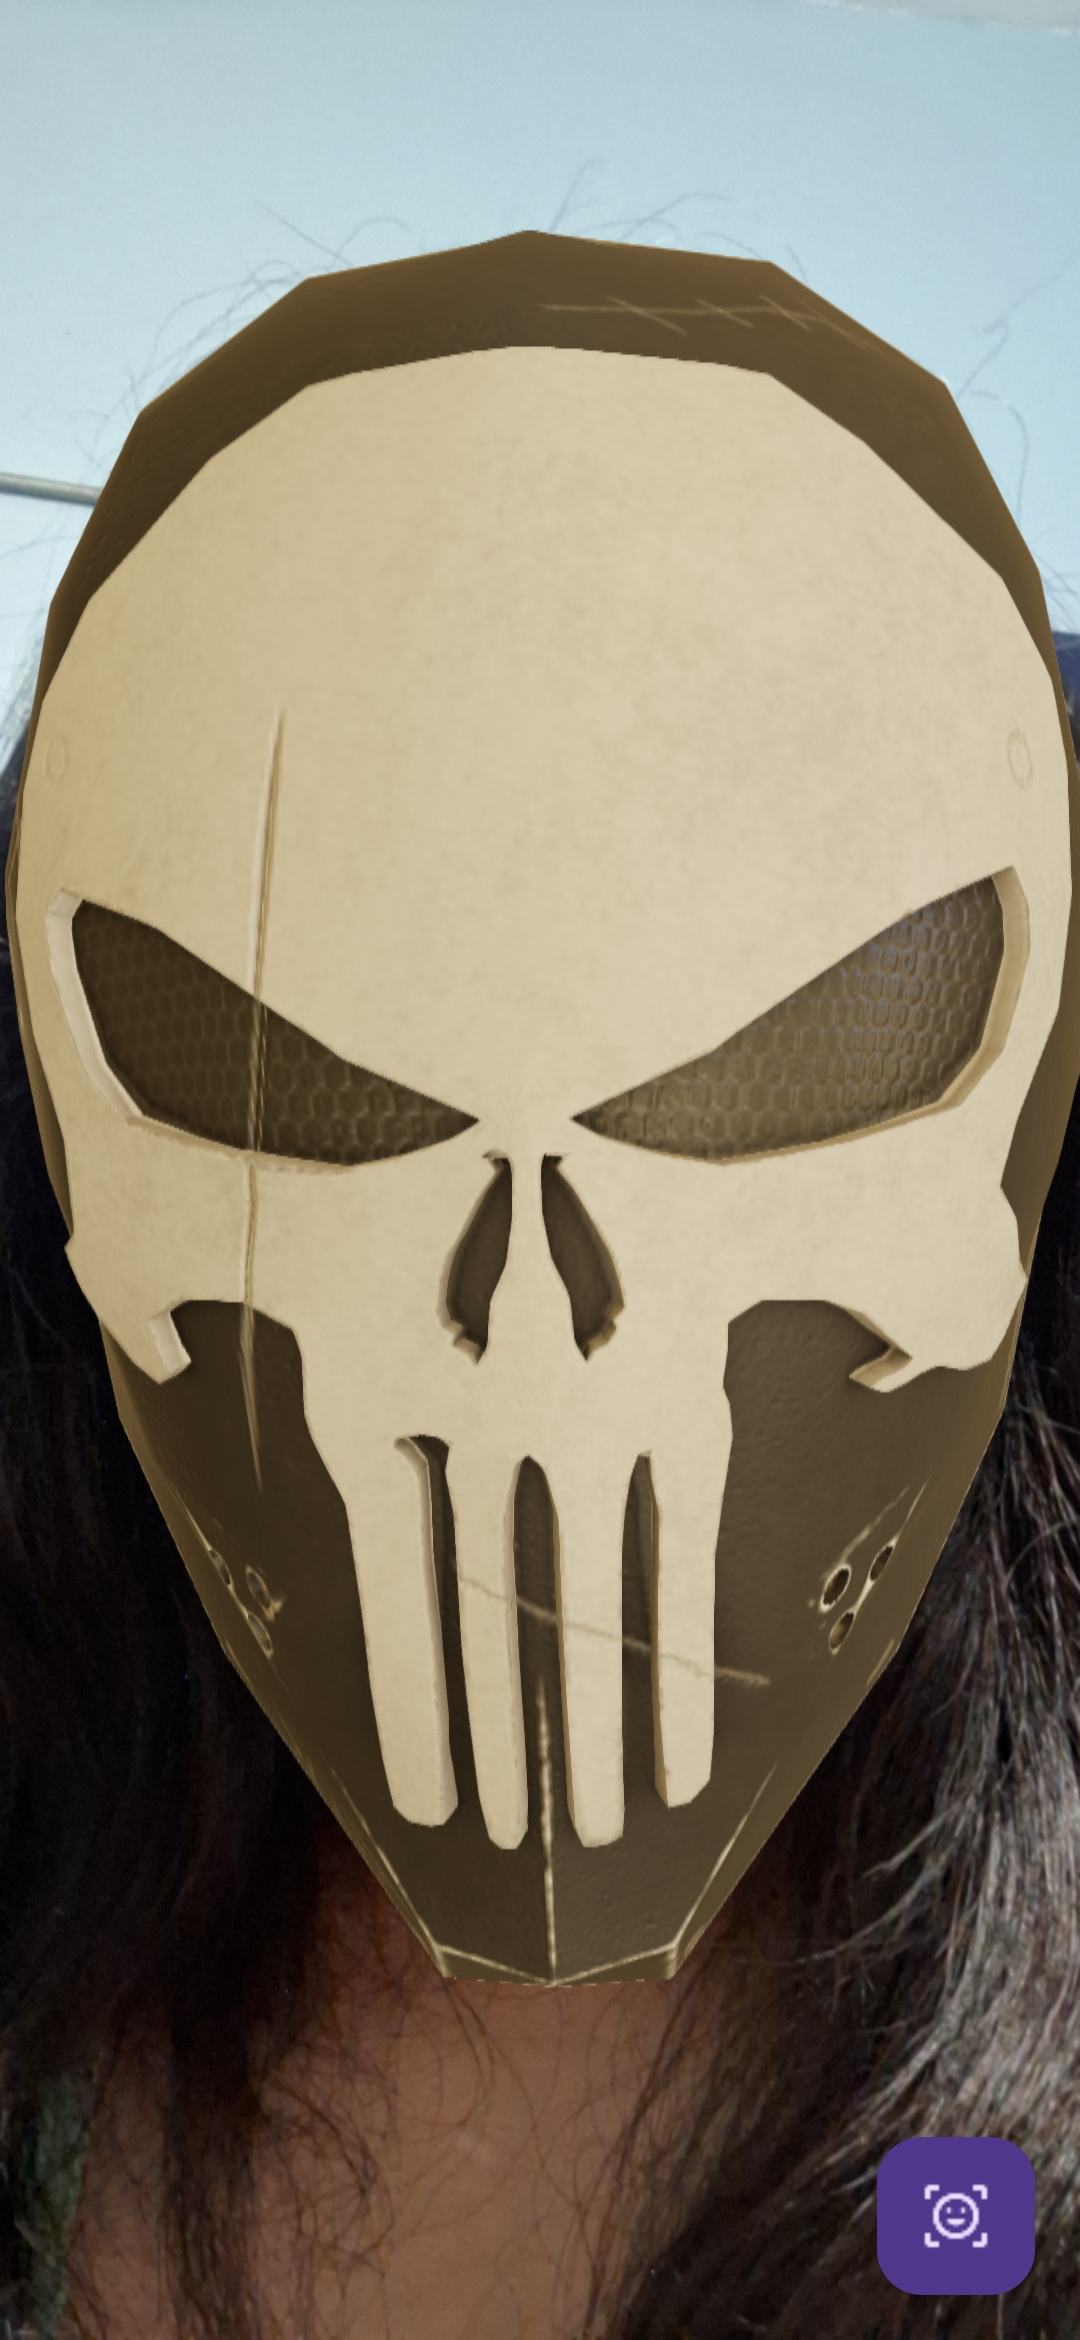
\includegraphics[width=0.3\linewidth]{images/mascara.jpg}%
            }\quad
            \subfloat[Cabeza de mario]{%
                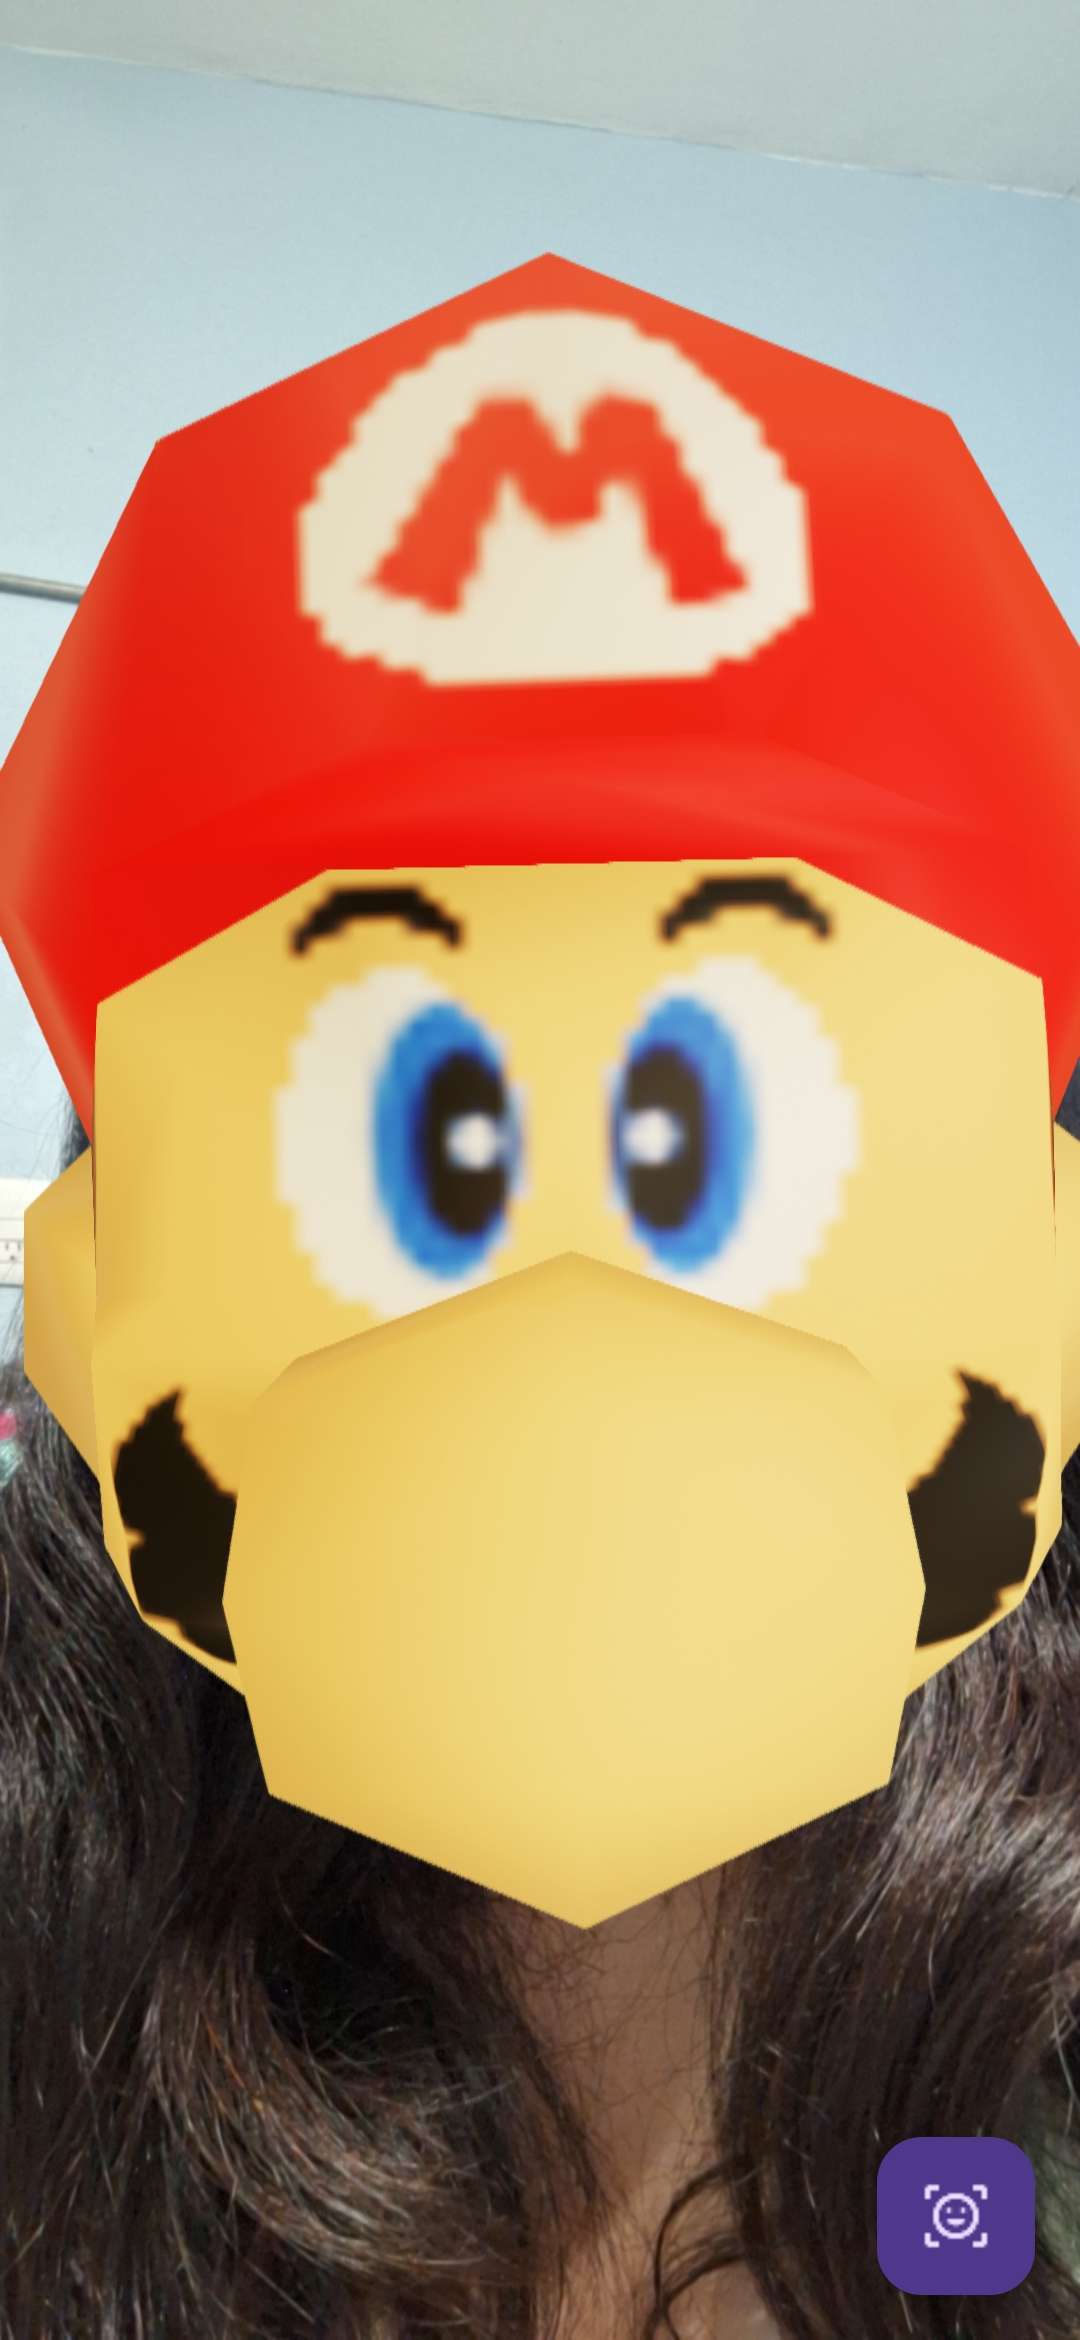
\includegraphics[width=0.3\linewidth]{images/cabeza.jpg}%
            }\quad
            \subfloat[Casco vintage]{%
                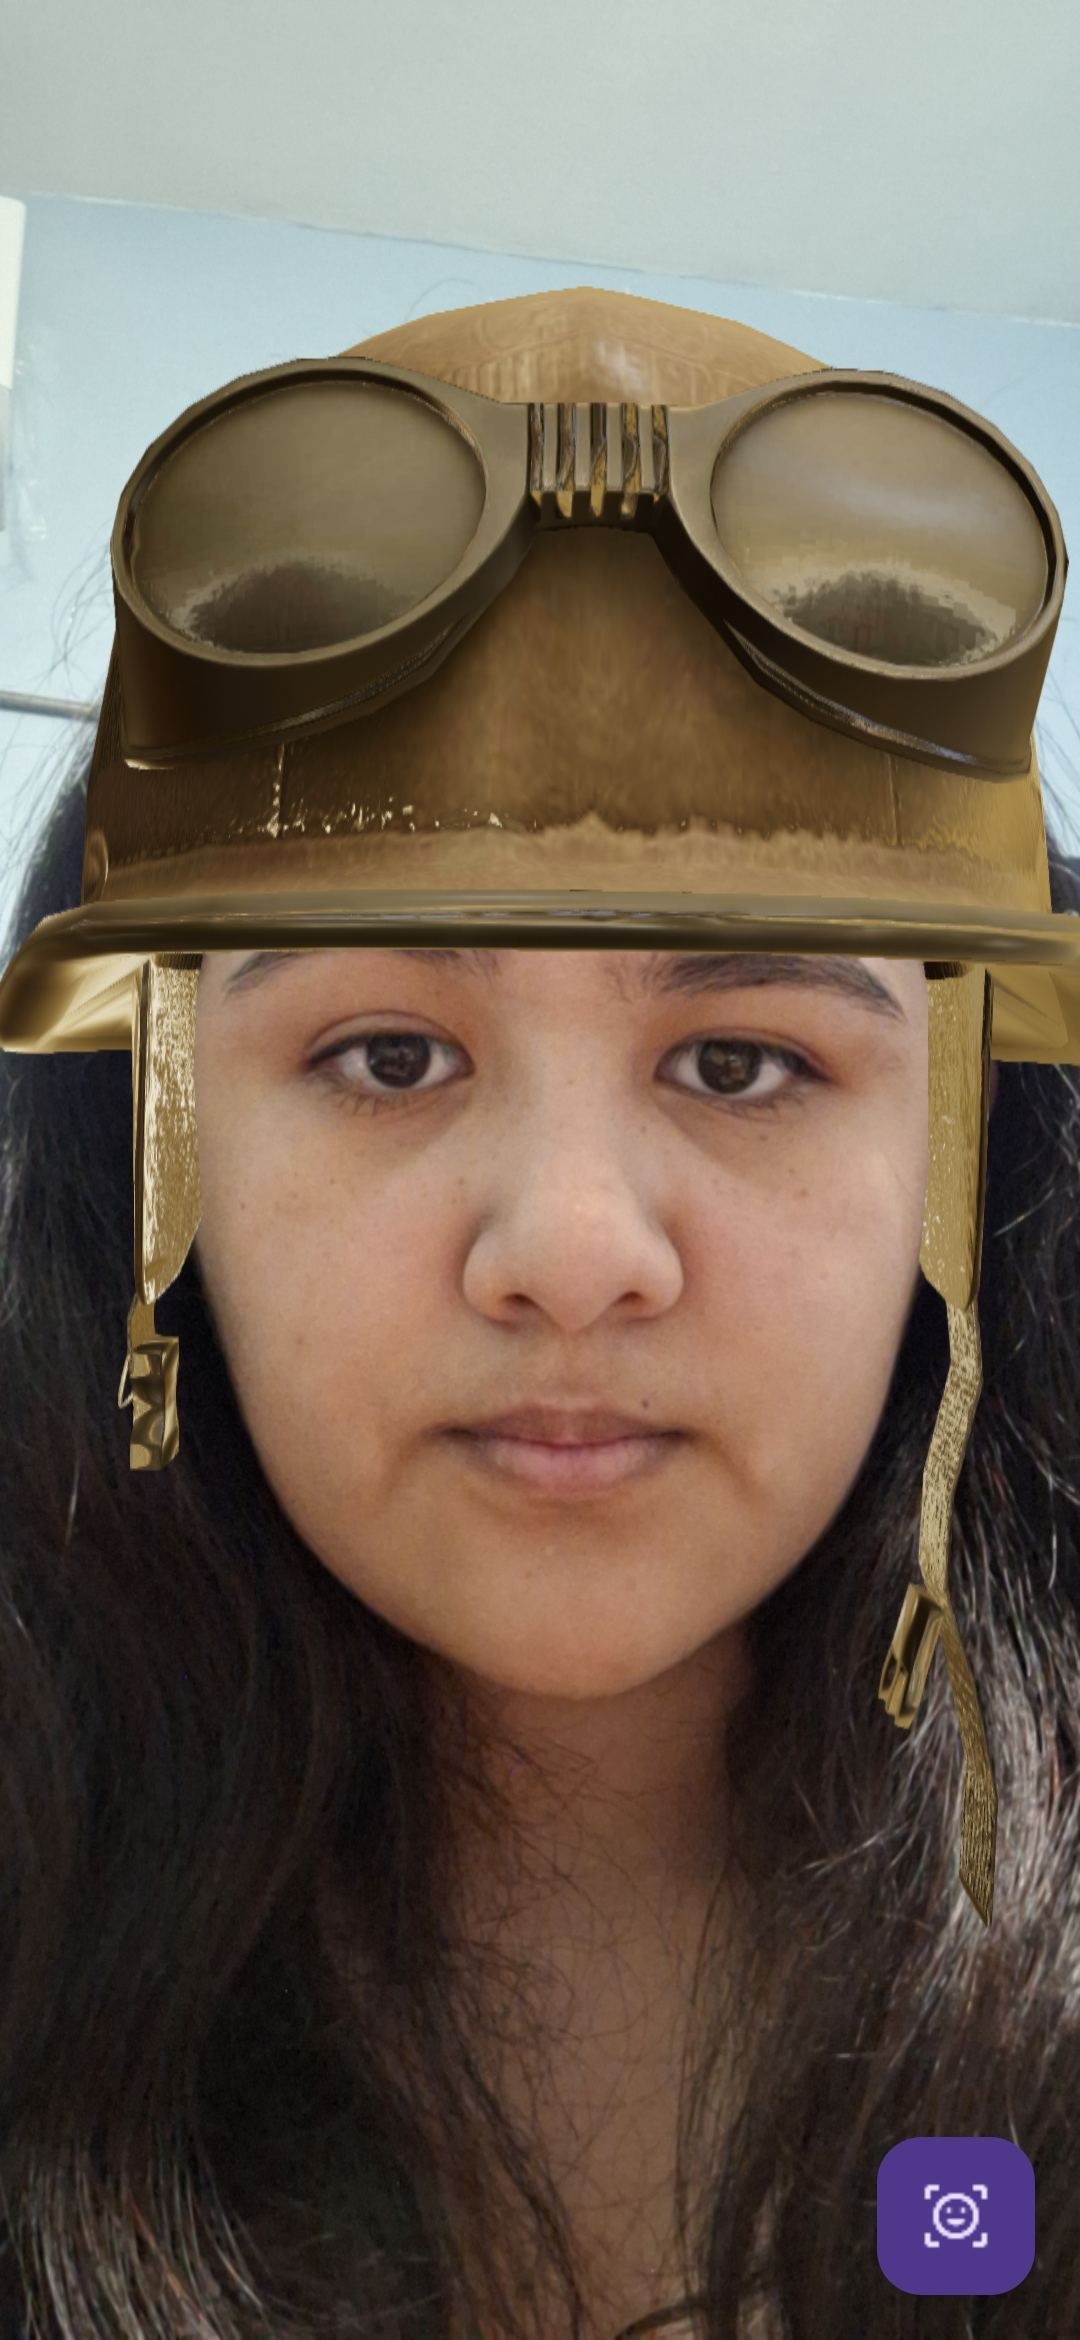
\includegraphics[width=0.3\linewidth]{images/casco.jpg}%
            }
            \caption{Modelos 3D superpuestos en un rostro. La figura (a) muestra una máscara simple, (b) una cabeza de un personaje y (c) un casco. Estos ejemplos demuestran la variedad de elementos que la aplicación puede renderizar.}
        \end{figure}

    \subsection{Menú de selección}
        El menú de selección se diseñó para que fuera fácil de usar. Cuando el usuario selecciona un modelo, la aplicación envia esta información a la pantalla principal para que el modelo se aplique inmediatamente. El resultado fue una navegación simple e intuitiva para el usuario.
        \begin{figure}[h!]
            \centering
            \subfloat[Menú de modelos]{%
                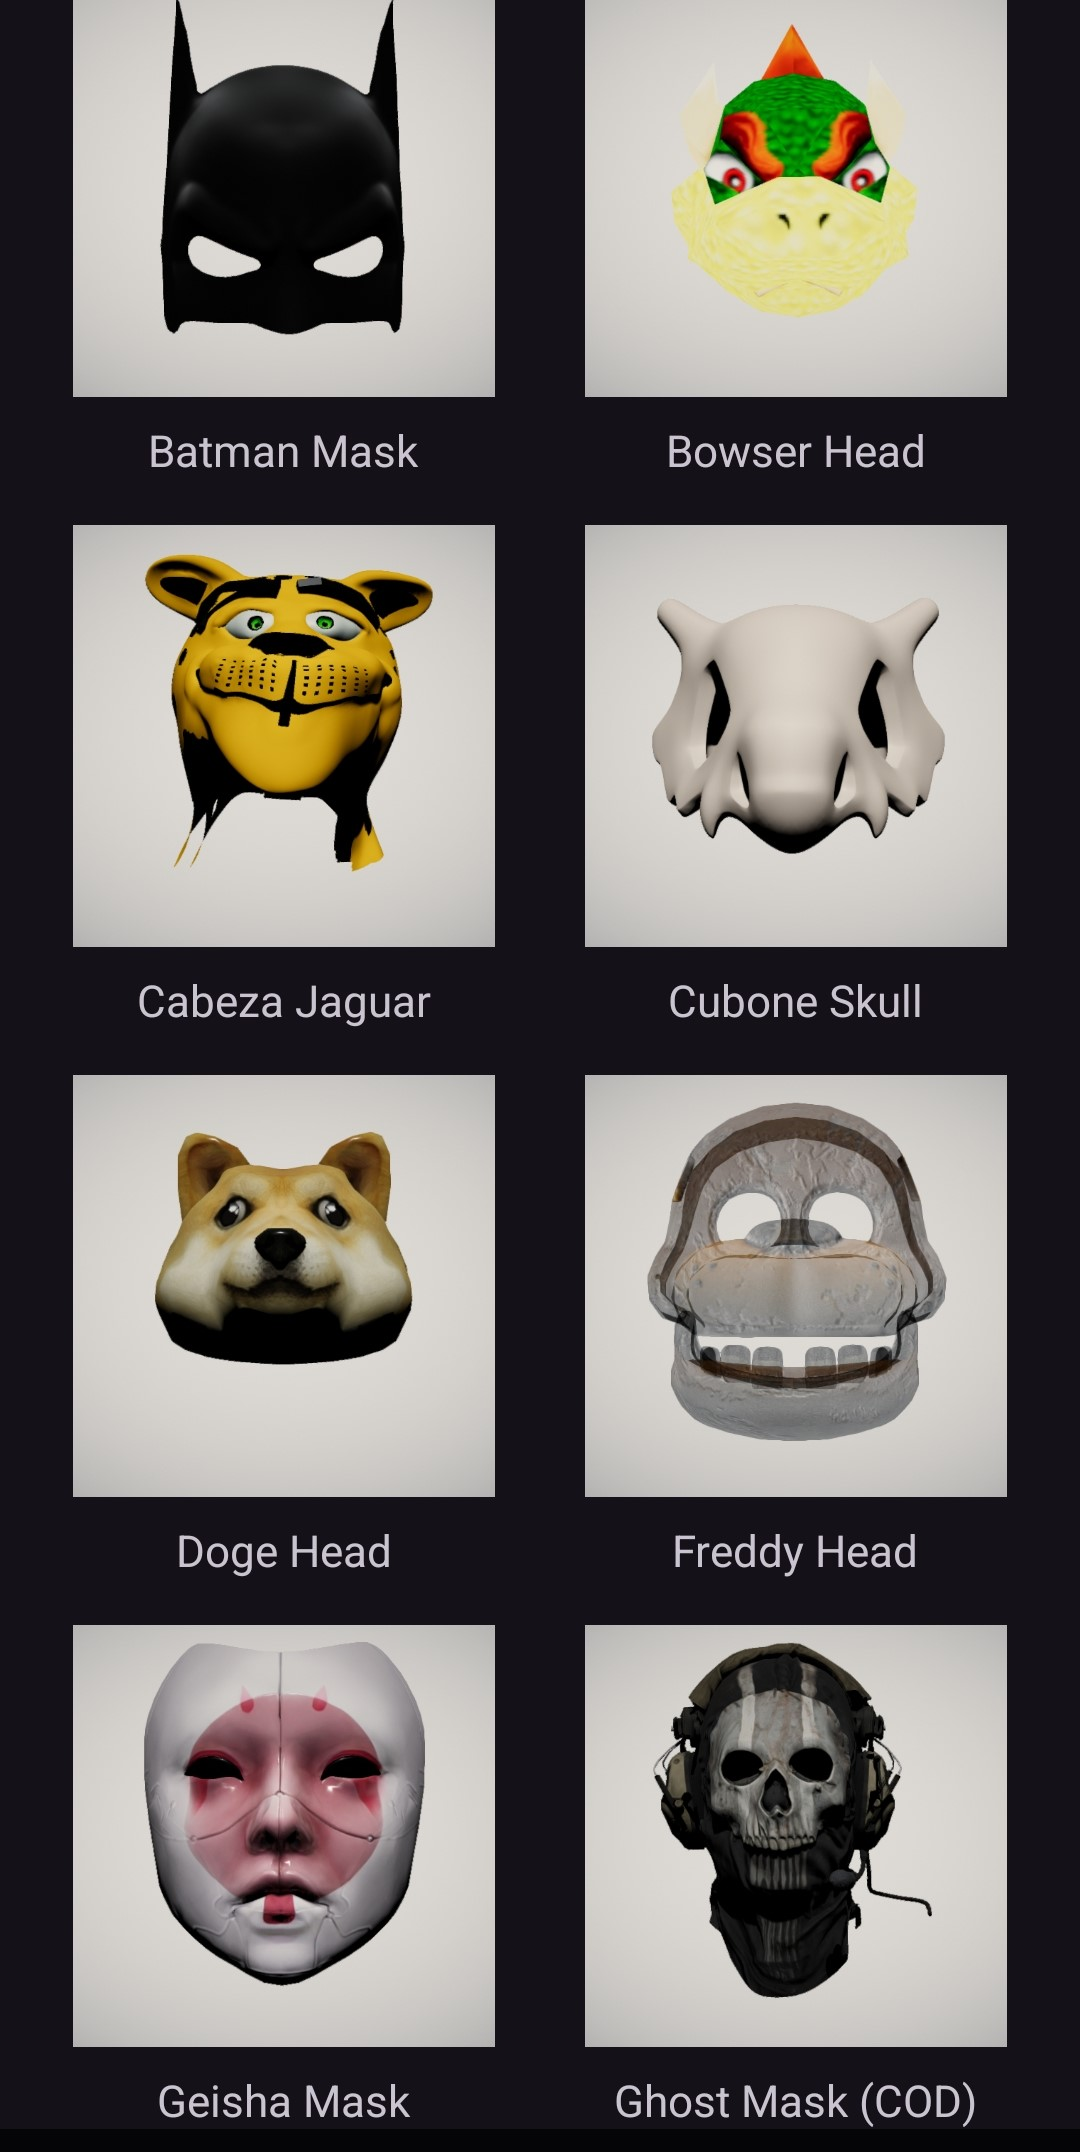
\includegraphics[width=0.3\linewidth]{images/modelos.jpg}%
            }\quad
            \subfloat[Menú de modelos 2]{%
                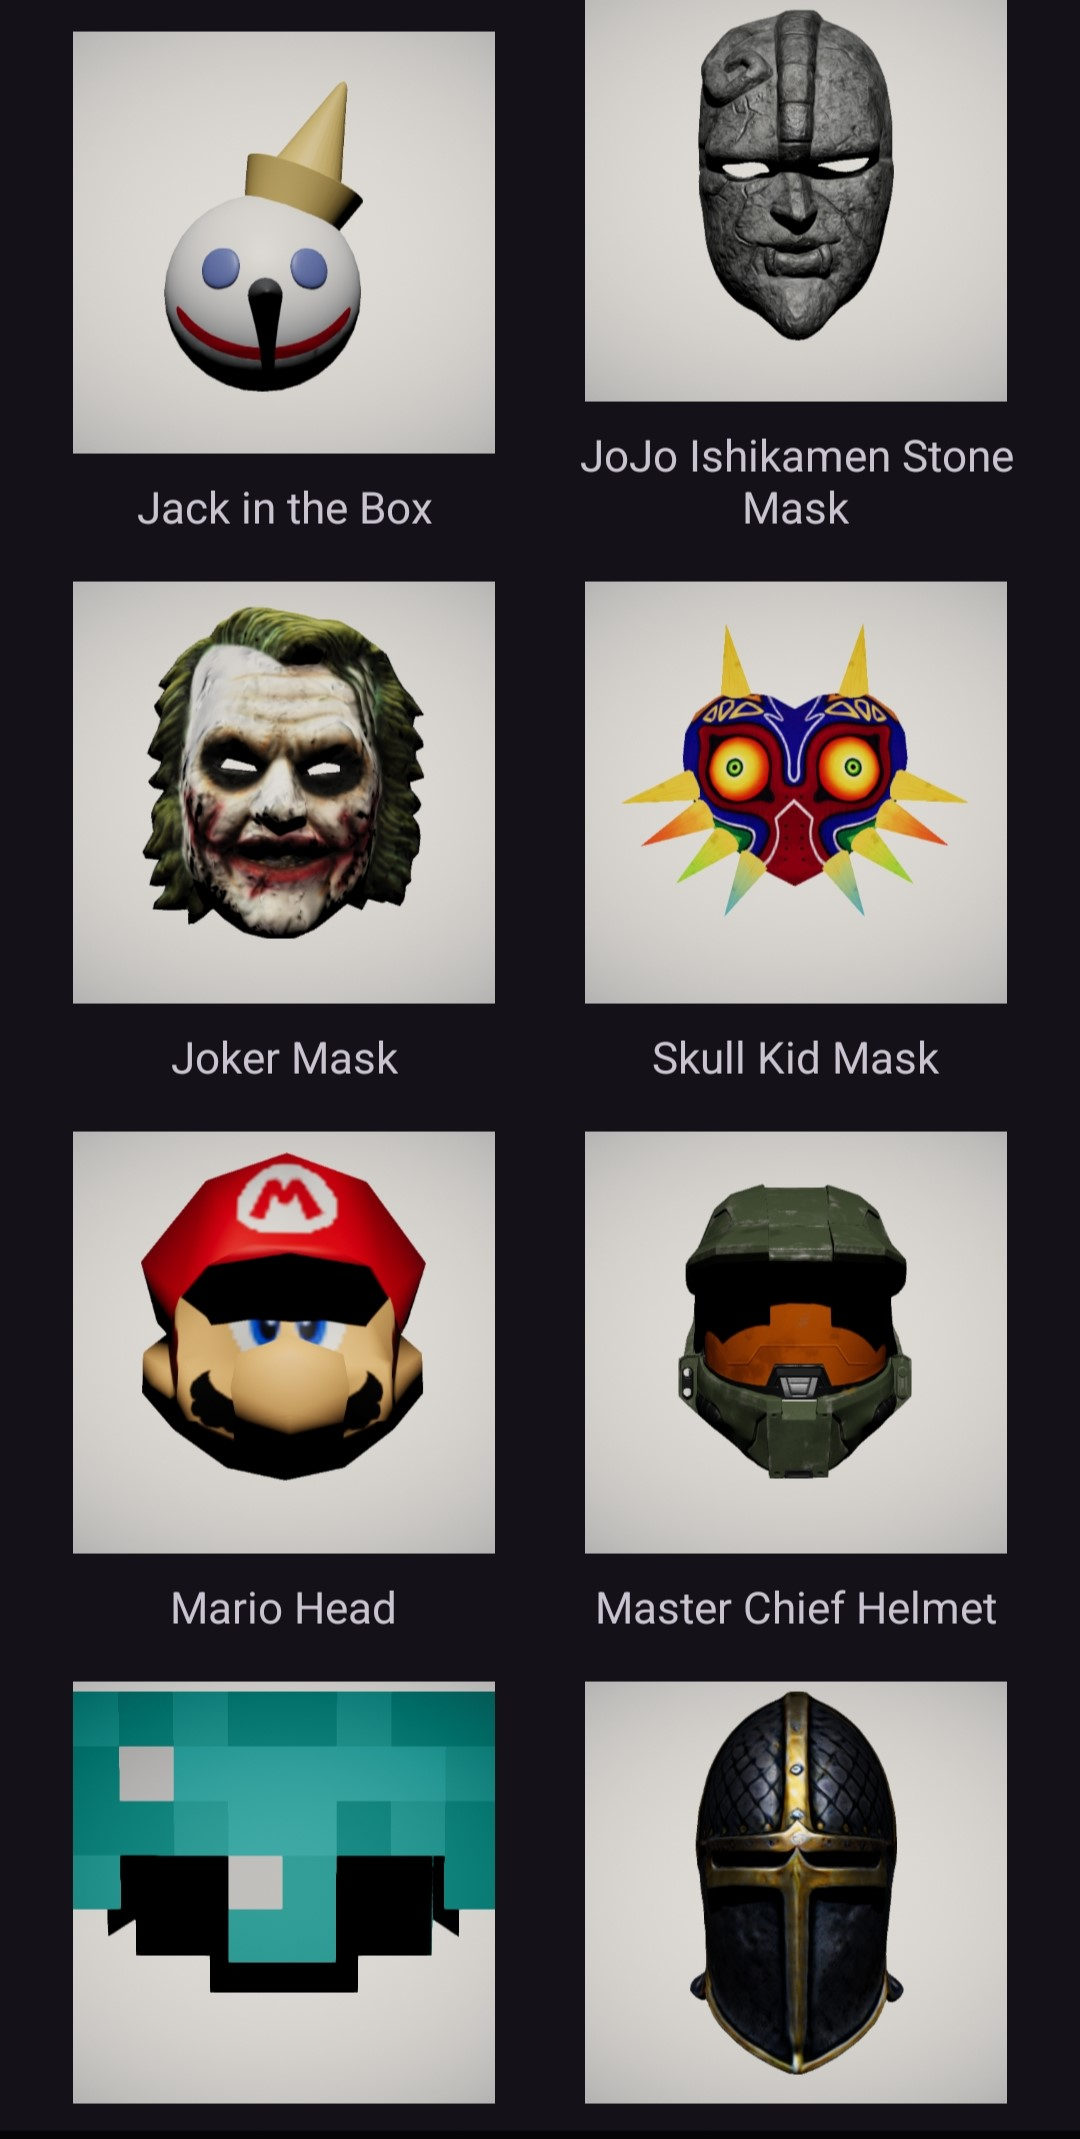
\includegraphics[width=0.3\linewidth]{images/modelos2.jpg}%
            }\quad
            \subfloat[Selección de un modelo]{%
                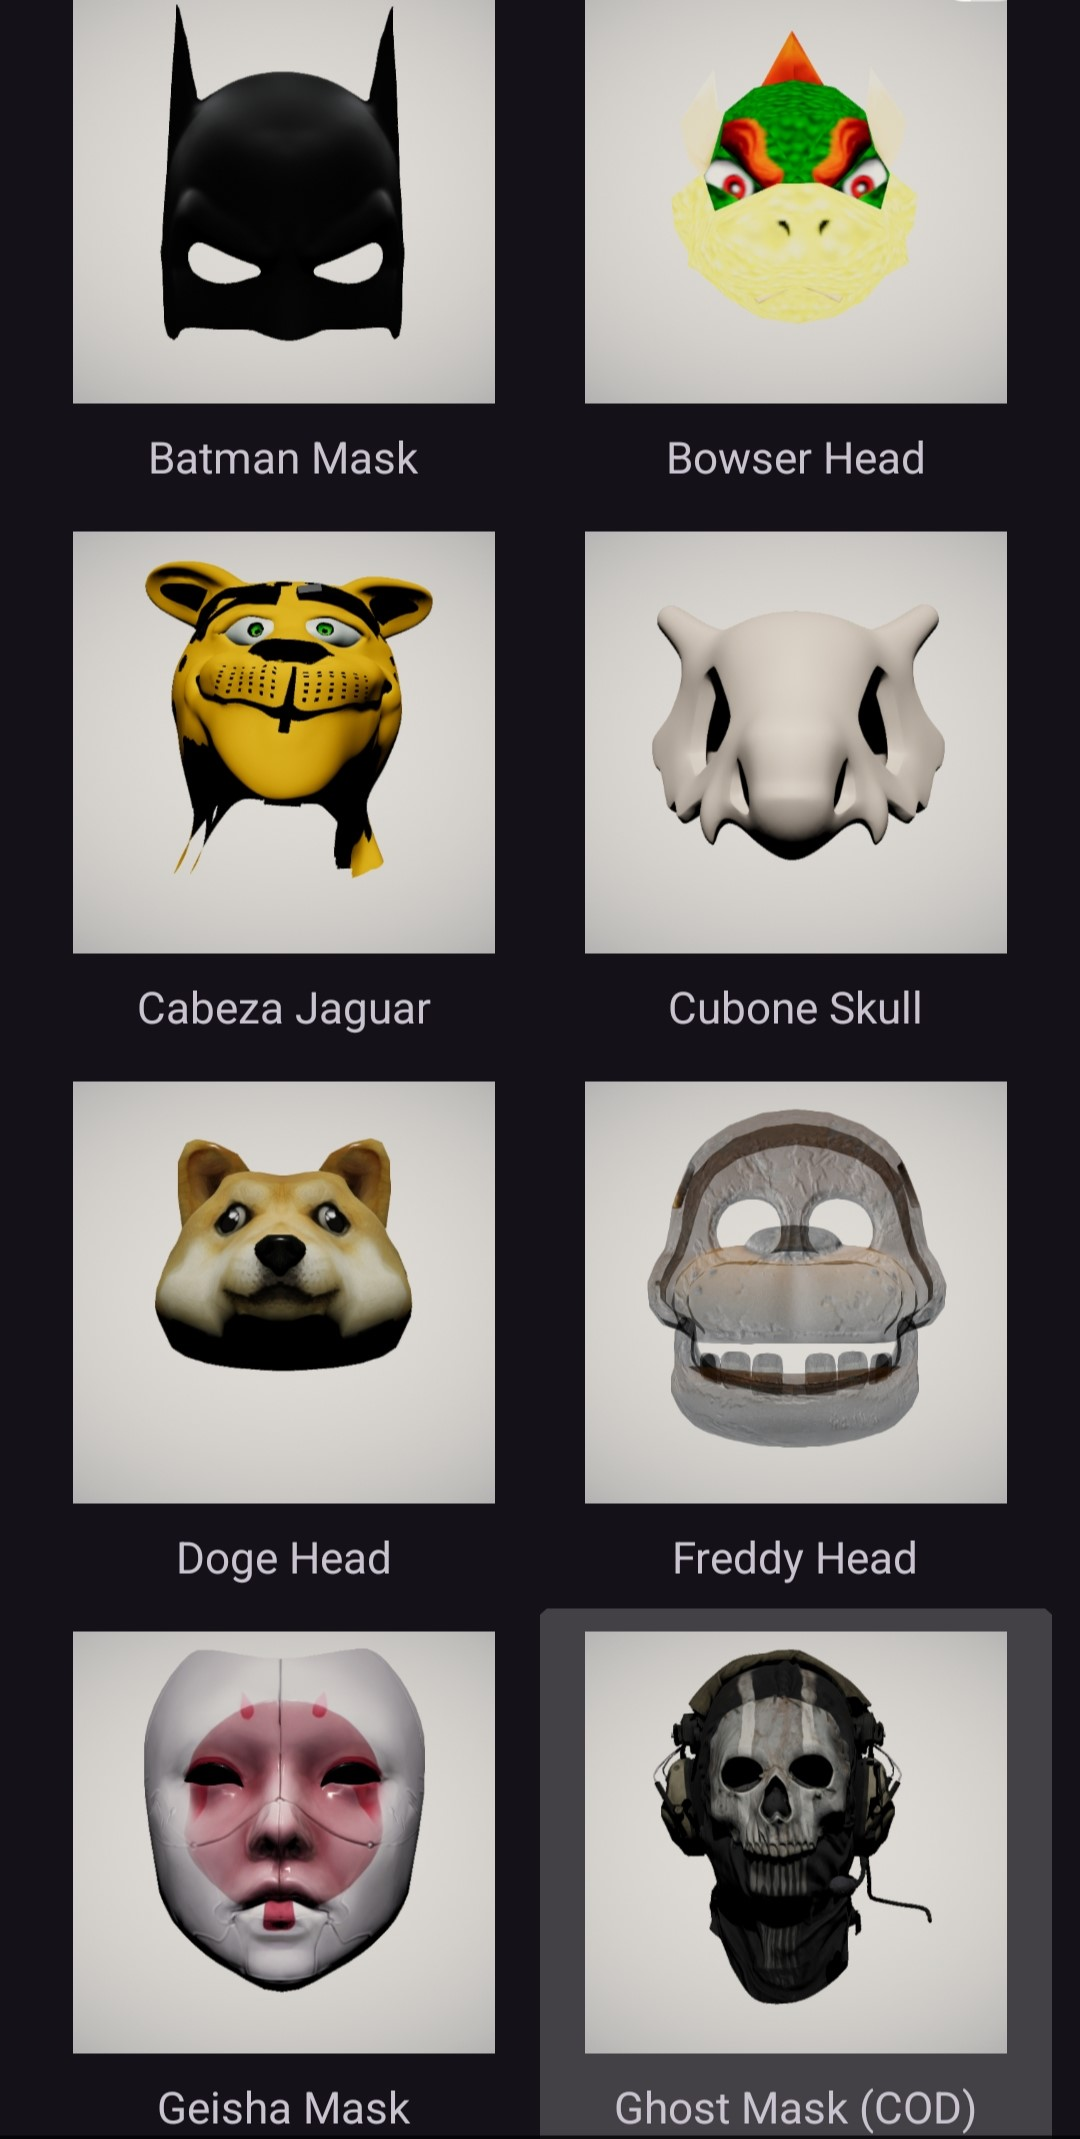
\includegraphics[width=0.3\linewidth]{images/seleccion.jpg}%
            }
            \caption{Interfaz del menú de selección de modelos. La figura (a) muestra el menú principal, (b) la continuación de la lista de modelos y (c) la selección de un modelo.}
        \end{figure}

    
    \subsection{Seguimiento de rostros y superposición de RA}
        La aplicación usa la cámara frontal para detectar un rostro y, una vez encontrado, lo segue de manera precisa. El sistema puede seguir la rotación y posición con precisión. Si un rostro deja de verse, el modelo 3D asociado desaparece, liberando recursos.
        \begin{figure}[h!]
            \centering
            \subfloat[De frente]{%
                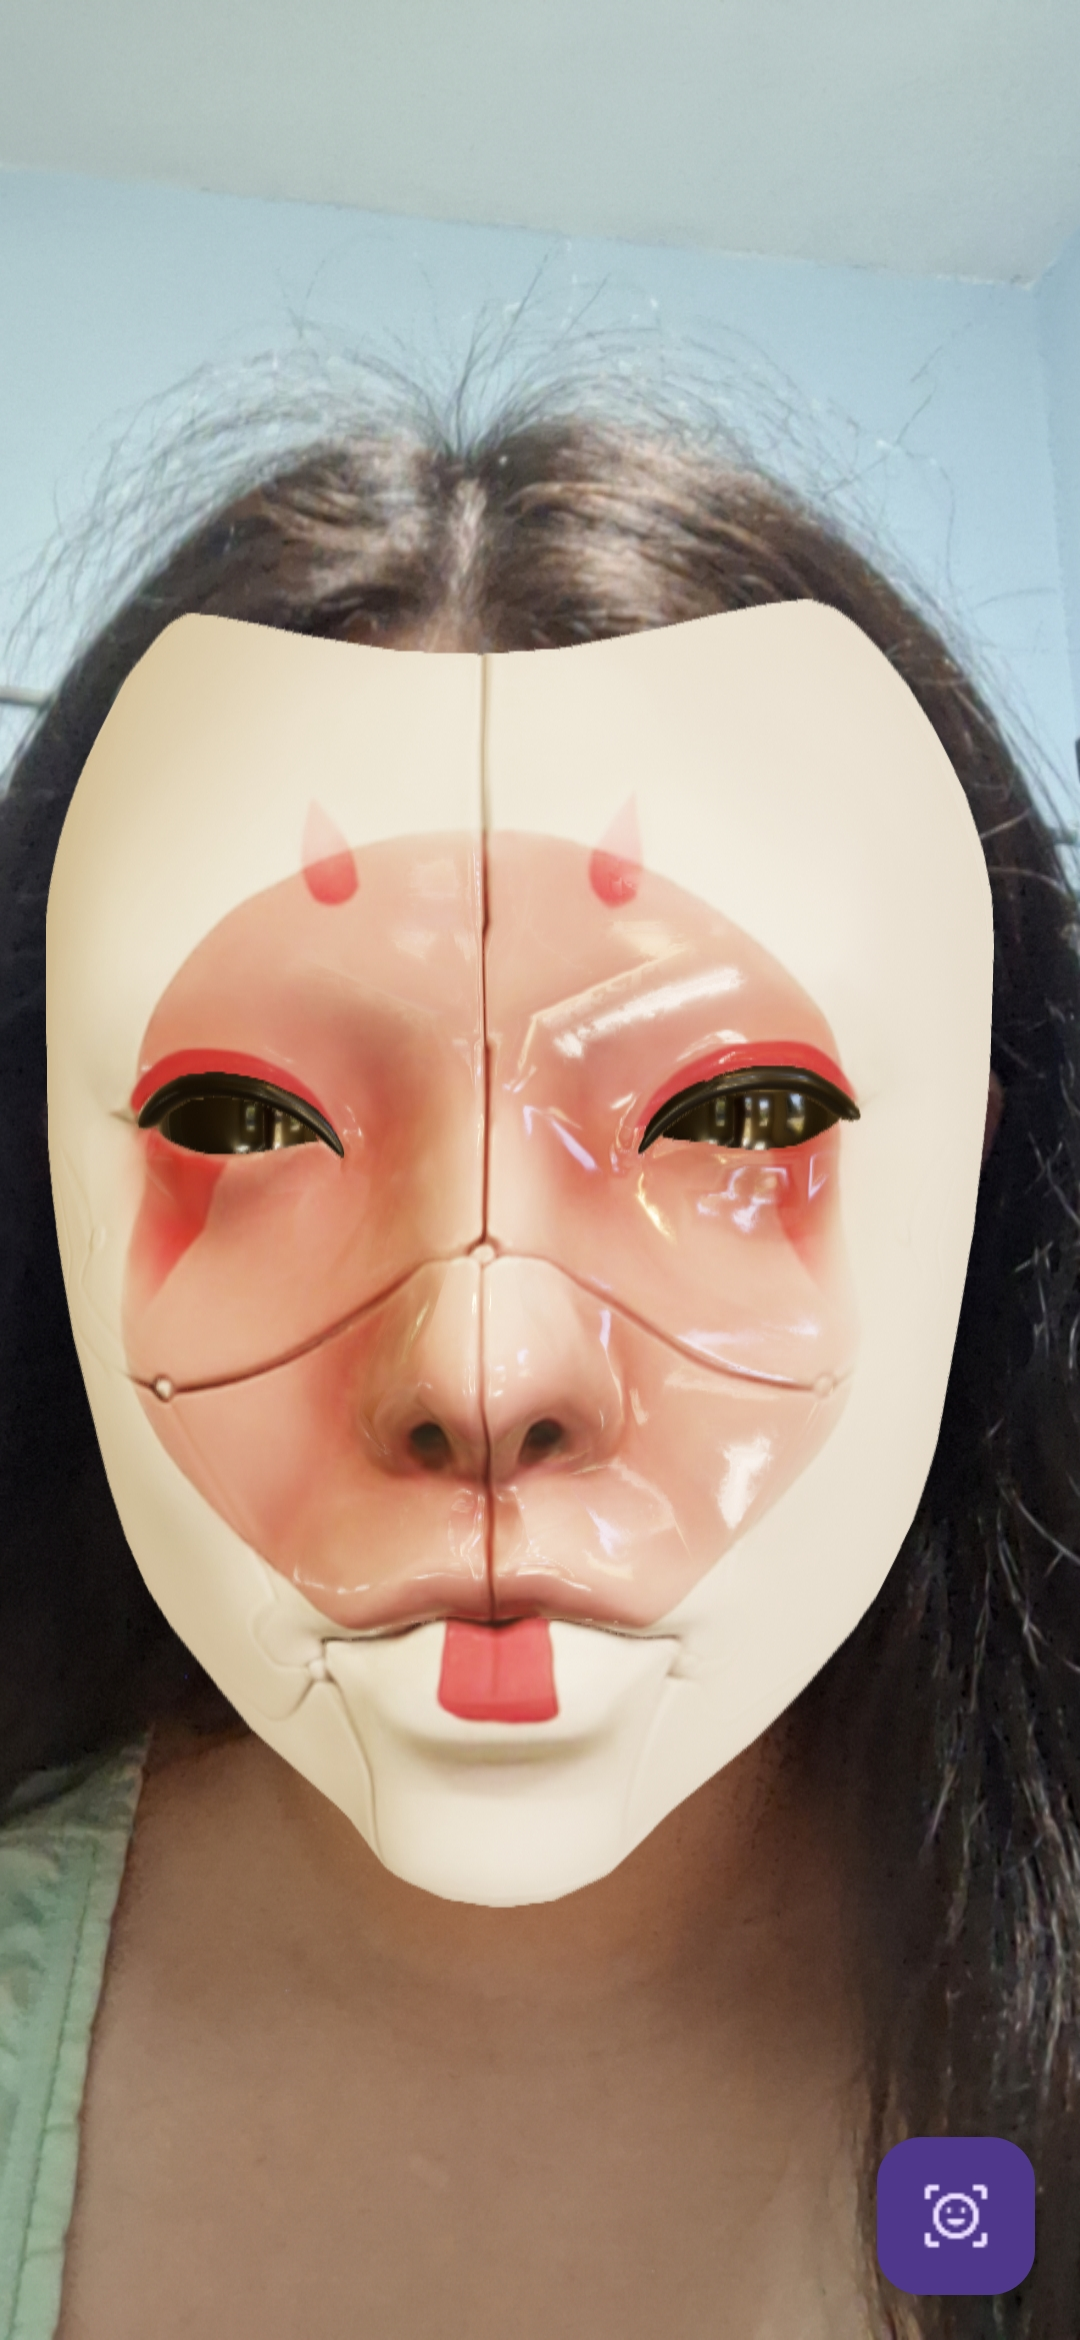
\includegraphics[width=0.3\linewidth]{images/frente.jpg}%
            }\quad
            \subfloat[De lado]{%
                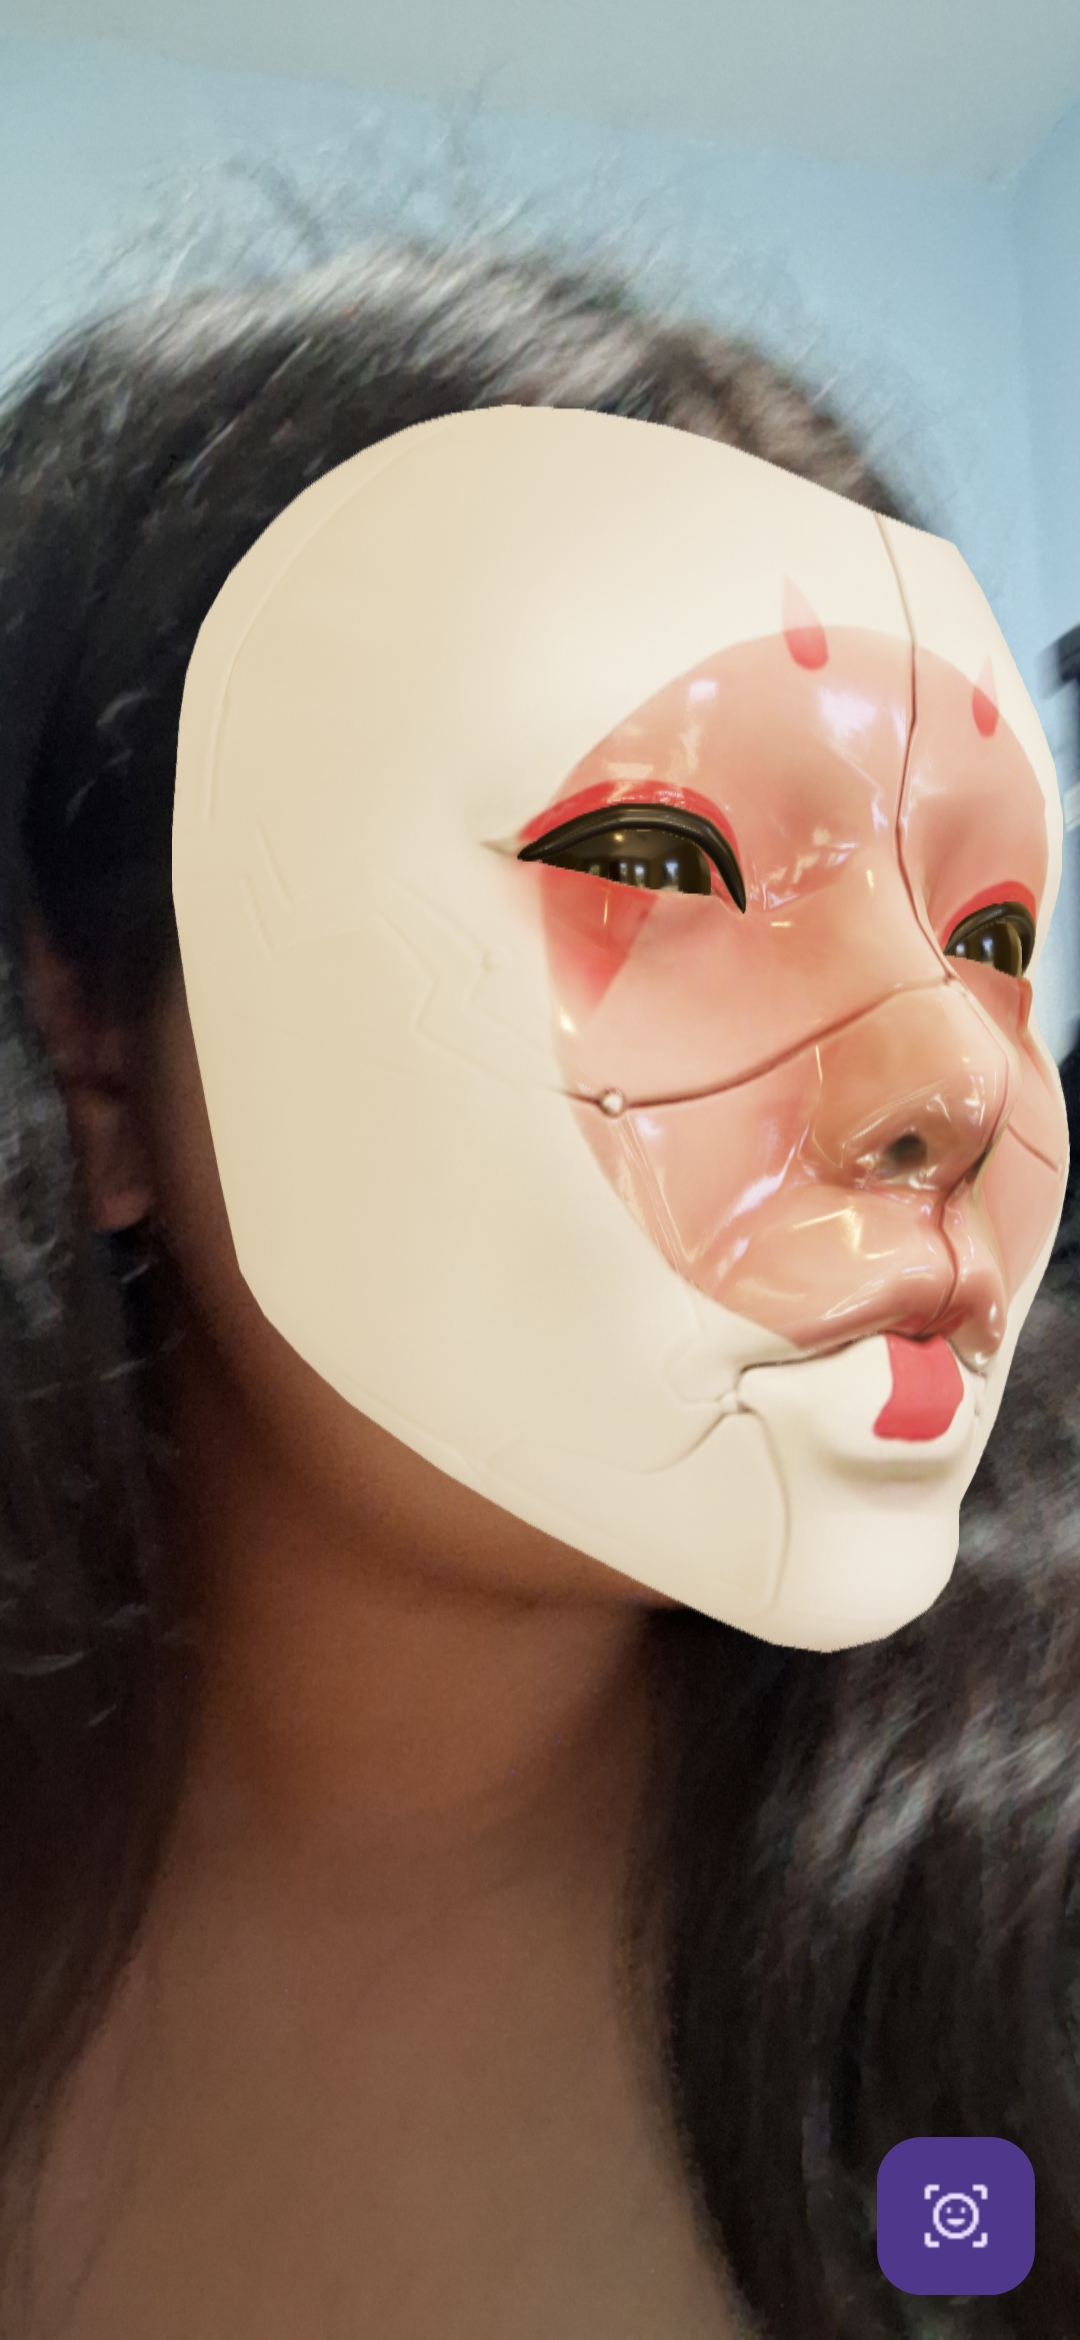
\includegraphics[width=0.3\linewidth]{images/lado.jpg}%
            }\quad
            \subfloat[Mirando arriba]{%
                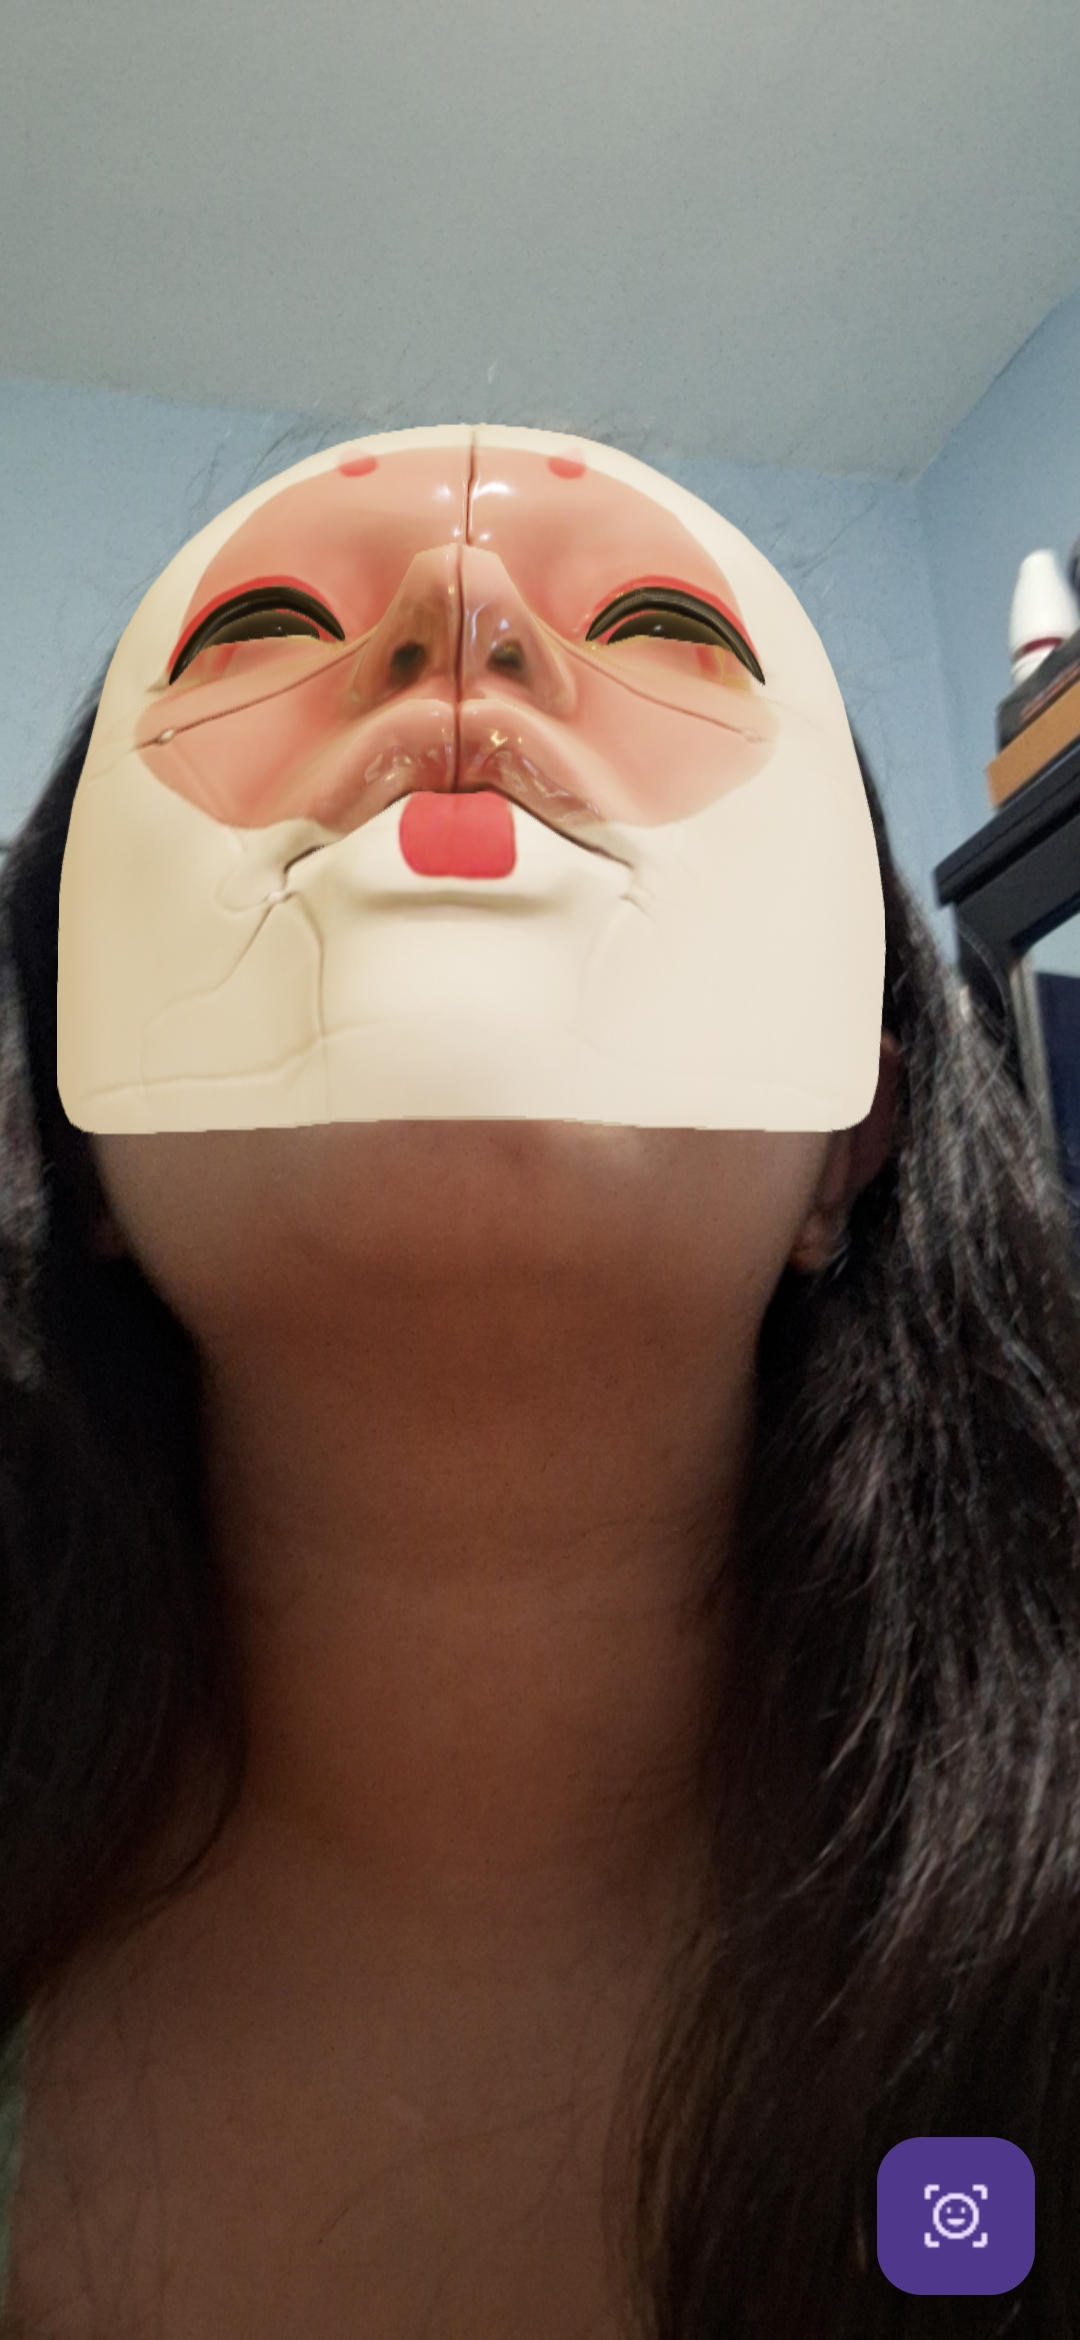
\includegraphics[width=0.3\linewidth]{images/arriba.jpg}%
            }
            \caption{Ejemplos del seguimiento de rostros en tiempo real. La figura (a) muestra la detección inicial, (b) el seguimiento con movimiento de cabeza y (c) el seguimiento con otro movimiento.}
        \end{figure}


\section{Conclusión}

    En conclusión, el desarrollo de esta aplicación de Realidad Aumentada para Android, que permite superponer modelos 3D en rostros detectados, demuestra una integración exitosa de ARCore y Sceneform. El proceso abarcó desde la configuración técnica inicial y la implementación del seguimiento de rostros en tiempo real y la carga asíncrona de modelos, hasta la creación de una interfaz de usuario para la selección de modelos. La interconexión de archivos java a través de mecanismos como listeners e intents fue fundamental para lograr una experiencia de Realidad Aumentada funcional y reactiva, ofreciendo al usuario la capacidad de interactuar con modelos 3D superpuestos en sus rostros utilizando la cámara frontal del dispositivo.
    
\printbibliography

%Bibliografía, Julissa%


\end{document}
